% =====================================================================
% Soutenance de stage — Vadim Lagresle — Criteo AI Lab — septembre 2026
% Stabilisation et efficience de l'entraînement autonome des agents LLM
%
% Compilation : pdfLaTeX (Overleaf). Figures attendues dans figures/
% (copier docs/rapport/figures/*.pdf dans un dossier figures/ du projet).
% Palette inspirée de la charte Criteo : orange FE5000, anthracite 2A2E33,
% bleu 006CD6, gris clair F2F2F0. Police : Fira Sans (proche de Graphik).
% =====================================================================
\documentclass[aspectratio=169,10pt]{beamer}
\usepackage[utf8]{inputenc}
\usepackage[T1]{fontenc}
\usepackage[french]{babel}
\usepackage[sfdefault,light]{FiraSans}
\usepackage{amsmath,amssymb}
\usepackage{booktabs}
\usepackage{graphicx}
\usepackage{xcolor}
\usepackage{colortbl}
\usepackage{tikz}
\usepackage{appendixnumberbeamer}
\graphicspath{{figures/}{../rapport/figures/}}

% ---------- Palette ----------
\definecolor{crOrange}{HTML}{FE5000}
\definecolor{crDark}{HTML}{2A2E33}
\definecolor{crBlue}{HTML}{006CD6}
\definecolor{crGrey}{HTML}{F2F2F0}
\definecolor{crMid}{HTML}{8A8F96}

% ---------- Thème ----------
\usetheme{default}
\usecolortheme{seagull}
\setbeamertemplate{navigation symbols}{}
\setbeamercolor{normal text}{fg=crDark,bg=white}
\setbeamercolor{structure}{fg=crOrange}
\setbeamercolor{alerted text}{fg=crOrange}
\setbeamercolor{frametitle}{fg=crDark,bg=white}
\setbeamerfont{frametitle}{size=\Large,series=\bfseries}
\setbeamercolor{block title}{fg=white,bg=crOrange}
\setbeamercolor{block body}{fg=crDark,bg=crGrey}
\setbeamerfont{block title}{series=\bfseries}
\setbeamercolor{item}{fg=crOrange}
\setbeamertemplate{itemize items}{\raisebox{0.15ex}{\tikz\fill[crOrange] (0,0) rectangle (0.5ex,0.5ex);}}
\setbeamertemplate{enumerate items}[default]
\setbeamercolor{enumerate item}{fg=crOrange}
\setbeamercolor{caption name}{fg=crMid}
\setbeamertemplate{blocks}[rounded=false]

% Titre de slide : texte anthracite + court trait orange dessous
\setbeamertemplate{frametitle}{%
  \vspace{0.3cm}%
  \begin{minipage}{\dimexpr\textwidth}
    \usebeamerfont{frametitle}\usebeamercolor[fg]{frametitle}\insertframetitle\par
    \vspace{0.08cm}\textcolor{crOrange}{\rule{1.6cm}{2.2pt}}
  \end{minipage}\vspace{0.05cm}}

% Pied de page : ligne fine, nom, titre court, numéro
\setbeamertemplate{footline}{%
  \vbox{%
    \hbox to \paperwidth{\hskip0.9cm\textcolor{crOrange}{\rule{\dimexpr\paperwidth-1.8cm\relax}{0.6pt}}\hfil}%
    \vskip 3pt
    \hbox to \paperwidth{\hskip0.9cm{\scriptsize\textcolor{crMid}{Vadim Lagresle \;·\; Stabilisation et efficience de l'entraînement autonome des agents LLM \;·\; Criteo AI Lab}}\hfil{\scriptsize\textcolor{crMid}{\insertframenumber}}\hskip0.9cm}%
    \vskip 3pt}}

% Pages de section : fond orange, texte blanc
\newif\ifinappendix
\AtBeginSection[]{%
  \begingroup
  \setbeamercolor{background canvas}{bg=crOrange}
  \setbeamertemplate{footline}{}
  \begin{frame}[plain]
    \vfill
    \begin{minipage}{0.85\textwidth}
      {\color{white}\scriptsize\bfseries \ifinappendix ANNEXE\else PARTIE \thesection\fi}\\[0.3cm]
      {\color{white}\huge\bfseries\insertsectionhead}\\[0.4cm]
      {\color{white}\rule{2.4cm}{2.5pt}}
    \end{minipage}
    \vfill
  \end{frame}
  \endgroup}

% ---------- Macros ----------
\newcommand{\refs}[1]{\vfill{\tiny\textcolor{crMid}{Réfs : #1}}}
\newcommand{\kpi}[2]{{\color{crOrange}\fontsize{30}{32}\selectfont\bfseries #1}{\color{crOrange}\large\bfseries #2}}
\newcommand{\hl}[1]{\textcolor{crOrange}{\textbf{#1}}}
\newcommand{\cok}{\textcolor{crOrange}{\large$\bullet$}}
\newcommand{\cno}{\textcolor{crMid}{\large$\circ$}}
\newcommand{\chalf}{\textcolor{crBlue}{\large$\bullet$}}
\newenvironment{keymsg}{\begin{beamercolorbox}[sep=6pt,wd=\textwidth]{block body}\small}{\end{beamercolorbox}}

\title{Stabilisation et efficience de l'entraînement autonome des agents LLM}
\subtitle{Apprentissage par renforcement multi-tour sur TextCraft}
\author{Vadim Lagresle}
\institute{Criteo AI Lab \;·\; Soutenance de stage}
\date{Septembre 2026}

\begin{document}

% =====================================================================
% Page de titre : fond anthracite, titre orange
{
\setbeamercolor{background canvas}{bg=crDark}
\setbeamertemplate{footline}{}
\begin{frame}[plain]
  \vspace{0.5cm}
  \begin{minipage}{0.88\textwidth}
    {\color{crOrange}\rule{2.4cm}{3pt}}\\[0.4cm]
    {\color{white}\fontsize{24}{28}\selectfont\bfseries Stabilisation et efficience\\ de l'entraînement autonome\\ des agents LLM\par}
    \vspace{0.45cm}
    {\color{white}\large Apprentissage par renforcement multi-tour sur TextCraft\par}
    \vspace{1.1cm}
    {\color{white}\bfseries Vadim Lagresle}\\[0.1cm]
    {\color{crMid}\small Stage de fin d'études du Master MVA, ENS Paris-Saclay, réalisé au Criteo AI Lab}\\[0.1cm]
    {\color{crMid}\small Encadrants : Alberto Lumbreras, Patrick Gallinari, Alain Rakotomamonjy, Sylvain Lamprier}\\[0.1cm]
    {\color{crMid}\small Soutenance de stage \;·\; Septembre 2026}
  \end{minipage}
  \vfill
  \begin{minipage}{\textwidth}
    \IfFileExists{logos/criteo.png}{
\includegraphics[height=0.55cm]{logos/criteo.png}}{\textcolor{crMid}{[logo Criteo]}}%
    \hfill
    \IfFileExists{logos/mva.png}{\includegraphics[height=0.9cm]{logos/mva.png}}{\textcolor{crMid}{[logo MVA / ENS Paris-Saclay : logos/mva.png]}}%
  \end{minipage}
  \vspace{0.2cm}
\end{frame}
}

% =====================================================================
\begin{frame}{Sommaire}
\begin{enumerate}\setlength{\itemsep}{0.18cm}
  \item {\large\textbf{Sujet initial et littérature de départ}}\\
        {\color{crMid}\small L'auto-amélioration des LLM par leurs propres réponses, et pourquoi ça ne suffit pas pour des agents.}
  \item {\large\textbf{État de l'art des agents et recadrage}}\\
        {\color{crMid}\small Systèmes agentiques, environnements, trajectoires, RL interactif, curriculum. La question précise.}
  \item {\large\textbf{Banc d'essai : AgentGym-RL et TextCraft}}\\
        {\color{crMid}\small Pourquoi ce cadre, ce qu'il contient, ce que le papier laisse dans l'ombre.}
  \item {\large\textbf{Expériences et résultats}}\\
        {\color{crMid}\small Réplication, efficience avec LoRA, stabilité avec les curriculums, compute contrôlé.}
  \item {\large\textbf{Conclusion et perspectives}}\\
        {\color{crMid}\small Contributions, périmètre, directions.}
\end{enumerate}
\end{frame}

% =====================================================================
\section{Sujet initial et littérature de départ}


\begin{frame}{Sujet initial et littérature de départ}
\begin{block}{Sujet confié}
Auto-amélioration d'agents LLM par génération de données synthétiques et filtrage de préférences. Sujet exploratoire, avec pour horizon les agents de commerce de Criteo.
\end{block}
\vspace{0.2cm}
Quatre papiers fondateurs, quatre manières de se passer d'annotations :
\begin{itemize}
  \item \textbf{West-of-N} : améliorer le modèle de récompense par pseudo-préférences tirées des extrêmes de $N$ échantillons.
  \item \textbf{ScPO} : le vote majoritaire comme signal d'entraînement ; génération de nouveaux problèmes.
  \item \textbf{Coral} : deux agents en dialogue ; entraîner l'assertivité et la persuasion.
  \item \textbf{BOND} : distiller la distribution Best-of-$N$ dans la politique.
\end{itemize}
\vspace{0.2cm}
Point commun : le signal est fabriqué à partir des \emph{réponses} du modèle lui-même.
\refs{Pace et al. 2024 ; Prasad et al. 2024 ; Ni et al. 2025 ; Sessa et al. 2024 ; Wang et al. 2022 (Self-Consistency)}
\end{frame}

\begin{frame}{Limites de ces méthodes dans le cadre agentique}
\small
\begin{columns}[T]
\column{0.5\textwidth}
\textbf{Ce que ces méthodes supposent}
\begin{itemize}
  \item Une \emph{réponse} unique, produite en un tour.
  \item Plusieurs réponses à la \emph{même} question, comparables entre elles : une réponse finale identifiable pour le vote (ScPO), un score scalaire par un modèle de récompense pour le classement (West-of-N, BOND).
  \item Le signal porte sur la réponse finale, pas sur le chemin qui y mène.
\end{itemize}
\column{0.5\textwidth}
\textbf{Ce qu'un agent produit}
\begin{itemize}
  \item Une \emph{trajectoire} : actions et observations alternées sur des dizaines de tours.
  \item Des trajectoires qui ne se votent pas : deux chemins différents peuvent être justes, et il n'y a pas de « réponse finale » à comparer hors du succès.
  \item Une récompense terminale rendue par l'environnement ; un modèle de récompense sur trente tours n'est pas fiable.
\end{itemize}
\end{columns}
\vspace{0.15cm}
\begin{keymsg}
Décision commune avec les encadrants : rester sur des papiers académiques, comprendre d'abord ce qui fait apprendre un agent seul, avant les agents de commerce. D'où un travail de \hl{précision du périmètre}, qui fait partie du résultat.
\end{keymsg}
\end{frame}

% =====================================================================
\section{État de l'art des agents et recadrage}

\begin{frame}{Systèmes agentiques : définition et leviers d'amélioration}
\begin{columns}[T]
\column{0.55\textwidth}
Un LLM placé dans une boucle : il lit une observation, émet une action, reçoit la suivante.
\vspace{0.2cm}
\begin{itemize}
  \item \textbf{Harnais} : outils, mémoire, format d'action, gestion du contexte. L'agent n'est jamais évalué nu.
  \item \textbf{Poids} : la politique elle-même, ce que le modèle décide de faire à chaque tour.
  \item Une part importante de la performance vient du harnais, et le harnais lui-même s'optimise.
\end{itemize}
\column{0.42\textwidth}
\begin{block}{Trois leviers d'amélioration}
\begin{enumerate}
  \item Ingénierie du harnais.
  \item Calcul à l'inférence : échantillonner plus, réviser, voter.
  \item Optimisation des poids : apprendre de ses propres trajectoires.
\end{enumerate}
\end{block}
\end{columns}
\refs{Yao et al. 2023 (ReAct) ; Kimi K2.5 2026 ; Meta-Harness 2026 ; Toolathlon 2025}
\end{frame}

\begin{frame}{Environnements et bancs d'essai agentiques}
\begin{itemize}
  \item \textbf{Interactif} : l'agent observe les conséquences de ses actions.
  \item \textbf{Évolutif} : l'état change ; un benchmark figé ne le capture pas.
  \item \textbf{Multi-tour} : la difficulté vient de l'horizon, pas de chaque étape.
  \item \textbf{Récompense vérifiable} : un programme décide du succès, sans annotateur ni juge appris.
\end{itemize}
\vspace{0.3cm}
\begin{columns}[T]
\column{0.5\textwidth}
\begin{block}{Les bancs d'essai définissent les objectifs}
AgentGym (14 environnements), WebArena, ALFWorld, Toolathlon. Le banc dit ce qu'on attend d'un agent.
\end{block}
\column{0.5\textwidth}
\begin{block}{Toolathlon : la difficulté mesurée par l'horizon}
Outils logiciels réels, vérification du succès par exécution. Les tâches sont graduées par le nombre de tours qu'un modèle de référence met à les résoudre : l'horizon utile comme proxy de difficulté, idée que reprend notre curriculum Horizon.
\end{block}
\end{columns}
\refs{Xi et al. 2025 (AgentGym) ; Zhou et al. 2024 (WebArena) ; Shridhar et al. 2021 (ALFWorld) ; Toolathlon 2025}
\end{frame}

\begin{frame}{Trajectoires multi-tour : horizon, boucle fermée, attribution du mérite}
\begin{columns}[T]
\column{0.5\textwidth}
\textbf{Mono-tour et multi-tour}
\begin{itemize}
  \item Mono-tour : une question, une réponse, un verdict. Le cadre des maths et du code.
  \item Multi-tour en boucle ouverte : un plan complet, puis exécution sans retour.
  \item Multi-tour en boucle fermée : agir, observer, corriger. C'est là que vit l'agent.
  \item Le nombre de trajectoires possibles croît exponentiellement avec l'horizon $T$.
\end{itemize}
\column{0.5\textwidth}
\textbf{Ce qui rend l'apprentissage difficile}
\begin{itemize}
  \item Récompense terminale : un bit par épisode de trente tours. Aucune information sur quel tour a compté.
  \item Une trajectoire réussie avec des détours reçoit la même récompense qu'une trajectoire directe : les actions inutiles sont renforcées avec les bonnes.
  \item Un échec long punit toutes ses actions, y compris les bonnes intuitions.
  \item Peu d'information rétropropagée par unité de calcul.
\end{itemize}
\end{columns}
\refs{Sutton et Barto 2018 (attribution du mérite) ; Snell et al. 2024 ; Yao et al. 2023 (ReAct)}
\end{frame}

\begin{frame}{RL en environnement interactif : GRPO et grandeurs mesurées}
\begin{columns}[T]
\column{0.52\textwidth}
\small
\textbf{GRPO} : pour une tâche, $G$ trajectoires de récompenses $R_1,\dots,R_G$ ; avantage relatif au groupe
\[ \hat A_i = \frac{R_i - \operatorname{mean}(\mathbf R)}{\operatorname{std}(\mathbf R)+\delta} \]
\vspace{-0.3cm}

Pénalité KL vers une référence $\pi_{\text{ref}}$, coefficient $\beta$. Observations masquées du gradient.
\column{0.46\textwidth}
\small
\textbf{Trois grandeurs suivies sur tous les runs}
\begin{itemize}
  \item \hl{pass@1} sur les tâches de test : la performance.
  \item \hl{Entropie} de la politique : combien elle explore encore.
  \item \hl{KL} vers la référence : combien elle s'est éloignée.
\end{itemize}
\end{columns}
\vspace{0.15cm}
\begin{block}{Propriété centrale}
\small Un groupe tout réussi ou tout échoué a un avantage nul : \textbf{zéro gradient}. Seuls les groupes \emph{mixtes} apprennent. Un \emph{collapse} désigne le moment où la politique cesse d'explorer, ou s'éloigne de la référence sans retour.
\end{block}
\refs{Shao et al. 2024 (GRPO) ; Schulman et al. 2015, 2017 (TRPO, PPO) ; Cui et al. 2025 ; Liu et al. 2025 (Dr.~GRPO)}
\end{frame}

\begin{frame}{pass@$k$ et hypothèse du plafond}
\begin{columns}[T]
\column{0.55\textwidth}
\begin{itemize}
  \item \textbf{pass@1} : probabilité de réussir en un essai. \textbf{pass@$k$} : au moins une réussite sur $k$ essais.
  \item pass@$k$ du modèle nu mesure ce que le modèle \emph{sait déjà faire}, parfois.
  \item Yue et al. 2025 : à grand $k$, le modèle de base rattrape le modèle entraîné par RL. Le RL concentrerait la masse sur ce qui existait déjà.
\end{itemize}
\column{0.43\textwidth}
\begin{block}{Ce qu'on en retient}
pass@$k$ du modèle nu est une \textbf{borne haute plausible} de ce que le RL peut atteindre. La mesurer avant d'entraîner dit où la marge existe. ProRL, qui entraîne longtemps, observe que cette borne peut bouger.
\end{block}
\end{columns}
\refs{Yue et al. 2025 ; Chen et al. 2021 (estimateur pass@$k$) ; Liu et al. 2025 (ProRL) ; Brown et al. 2024 (Large Language Monkeys)}
\end{frame}

\begin{frame}{Curriculum, autocurriculum et agents autotéliques}
\footnotesize
\begin{itemize}\setlength{\itemsep}{2pt}
  \item \textbf{Curriculum} (Bengio 2009 ; Narvekar 2020) : tâches présentées par difficulté croissante, ordre \emph{fixé par l'humain}. Deux leviers : \hl{ordonner les tâches} ou \hl{doser les moyens} accordés pour les résoudre (horizon, budget).
  \item \textbf{Autocurriculum} (Portelas 2020) : la difficulté est choisie par un critère mesuré sur l'apprenant. Deux variantes :
  \begin{itemize}
    \item \emph{par progrès d'apprentissage} (Graves 2017) : proposer les tâches où la compétence bouge, ni les acquises ni les hors de portée ;
    \item \emph{agents autotéliques} : l'agent se donne ses buts dans un grand espace ; MAGELLAN (Gaven 2025) apprend un estimateur de compétence pour les choisir par progrès.
  \end{itemize}
\end{itemize}
\vspace{0.05cm}
\begin{block}{Intérêt dans notre cadre}
À récompense rare, une tâche hors de portée ne produit aucun signal, une tâche maîtrisée non plus. Le curriculum maintient l'apprenant là où le signal existe. Notre notion de difficulté n'est pas forcément celle du modèle : l'autocurriculum contourne la question en la mesurant.
\end{block}
\refs{Bengio 2009 ; Narvekar 2020 ; Portelas 2020 ; Graves 2017 ; Gaven 2025 (MAGELLAN)}
\end{frame}

\begin{frame}{Périmètre retenu et question de recherche}
\small
\begin{columns}[T]
\column{0.5\textwidth}
\textbf{Ce qu'on retient}
\begin{itemize}
  \item Le levier des \hl{poids}, par renforcement, en multi-tour.
  \item Un environnement \emph{donné}, à récompense vérifiable, léger, pour isoler les variables.
  \item Un petit modèle, un seul GPU : les contraintes réelles d'une équipe.
\end{itemize}
\column{0.5\textwidth}
\textbf{Ce qu'on laisse}
\begin{itemize}
  \item L'ingénierie du harnais et la mémoire.
  \item La fabrication d'environnements.
  \item Les agents de commerce eux-mêmes : c'est l'horizon, pas le terrain.
\end{itemize}
\end{columns}
\vspace{0.2cm}
\begin{block}{Question de recherche}
\normalsize Quelles conditions rendent l'entraînement par renforcement d'un agent LLM \textbf{stable} et \textbf{efficient} ?
\end{block}
\end{frame}

% =====================================================================
\section{Banc d'essai : AgentGym-RL et TextCraft}

\begin{frame}{Choix du banc d'essai : critères et candidats}
\scriptsize\setlength{\tabcolsep}{4pt}
\resizebox{\textwidth}{!}{%
\begin{tabular}{@{}lcccc@{}}
\toprule
\textbf{Critère (sections 2 et 3 du rapport)} & \textbf{Maths, code} & \textbf{WebArena} & \textbf{ALFWorld} & \textbf{TextCraft} \\
 & \tiny mono-tour, littérature initiale & \tiny \textbf{AgentGym-RL}, navigation web & \tiny AgentGym, embodied textuel & \tiny \textbf{AgentGym-RL}, crafting \\
\midrule
Interactif, multi-tour, boucle fermée & \cno & \cok & \cok & \cok \\
Récompense vérifiable exacte, sans juge appris & \cok & \chalf & \cok & \cok \\
Observabilité partielle & \cno & \cok & \cok & \cok \\
Difficulté paramétrable par construction & \chalf & \cno & \chalf & \cok \\
Simulateur léger, expériences répétées & \cok & \cno & \cok & \cok \\
Score publié sur un modèle de 3B & \cok & \cok & \cno & \cok \\
Recette d'entraînement publiée & \cok & \chalf & \chalf & \chalf \\
Plusieurs environnements, même plateforme & \cno & \cok & \cok & \cok \\
\bottomrule
\end{tabular}}
\hfill{\tiny\textcolor{crMid}{\cok\ oui \quad \chalf\ partiel \quad \cno\ non}}
\small
\vspace{0.2cm}
\begin{itemize}
  \item AgentGym-RL (Xi et al., ICLR 2026) : RL multi-tour, GRPO, Qwen2.5, curriculum ScalingInter ; WebArena et TextCraft en font partie, avec un score 3B publié pour chacun, mais une recette publiée pour le 7B seulement. Entre les deux, TextCraft l'emporte sur deux critères : la \hl{profondeur} de l'arbre de recette mesure la difficulté par construction, et le simulateur est assez léger pour répéter les expériences.
\end{itemize}
\refs{Xi et al. 2025 ; Prasad et al. 2023 (TextCraft) ; Zhou et al. 2024 (WebArena) ; Shridhar et al. 2021 (ALFWorld)}
\end{frame}

\begin{frame}{TextCraft : environnement, actions et jeu de données}
\begin{columns}[T]
\column{0.56\textwidth}
\begin{beamercolorbox}[sep=5pt,wd=\textwidth]{block body}
\scriptsize\ttfamily
You are given few useful crafting recipes to craft items in Minecraft. Crafting commands are of the format "craft [target object] using [input ingredients]". Every round I will give you an observation, you have to respond an action [\dots] You can "get" an object from the inventory or the environment, look-up the game inventory by "inventory", or "craft" (target) using any of the crafting commands. [\dots]\\[3pt]
\textbf{Goal: craft flint and steel.}
\end{beamercolorbox}
\vspace{0.2cm}
\small Trois actions : \texttt{get}, \texttt{craft}, \texttt{inventory}. Récompense 1 si l'objet est dans l'inventaire final, 0 sinon. Trente tours au plus.
\column{0.42\textwidth}
\small
\textbf{Profondeur} = hauteur de l'arbre de recette.\\[0.2cm]
{\footnotesize\setlength{\tabcolsep}{4pt}
\begin{tabular}{@{}lrrrr@{}}
\toprule
 & $d{=}1$ & $d{=}2$ & $d{=}3$ & $d{=}4$ \\
\midrule
Train (374) & 109 & 221 & 43 & \hl{1} \\
Test (100) & 31 & 41 & 25 & 3 \\
\bottomrule
\end{tabular}}
\vspace{0.3cm}
\begin{itemize}
  \item 544 recettes ; 70 réservées aux exemples few-shot, sans fuite.
  \item Une seule recette de profondeur 4 à l'entraînement : limite du jeu de données que le papier ne discute pas.
\end{itemize}
\end{columns}
\end{frame}

\begin{frame}{Résultats de référence sur TextCraft et oracle pass@$k$}
\begin{columns}[T]
\column{0.62\textwidth}
\footnotesize\setlength{\tabcolsep}{3.5pt}
\begin{tabular}{@{}lccccc@{}}
\toprule
\textbf{Modèle (\%, 100 tâches test)} & $d{=}1$ & $d{=}2$ & $d{=}3$ & $d{=}4$ & \textbf{Global} \\
\midrule
Qwen2.5-3B nu (papier) & 35 & 7 & 0 & 0 & 14 \\
Qwen2.5-3B nu (nous, 20 passes) & & & & & \hl{10,3} \\
Qwen2.5-7B nu & 81 & 41 & 0 & 0 & 42 \\
\rowcolor{crGrey}AgentGym-RL-3B (papier) & 100 & 90 & 28 & 0 & \textbf{75} \\
AgentGym-RL-7B (papier) & 100 & 98 & 72 & 0 & 89 \\
Qwen3.5-4B nu (nous, 18 passes) & & & & & 78,5 \\
GPT-4o & 100 & 88 & 64 & 0 & 83 \\
Gemini-2.5-Pro & 100 & 100 & 84 & 33 & 94 \\
\bottomrule
\end{tabular}
\column{0.36\textwidth}
\small
\textbf{Oracle pass@$k$ du 3B nu}
\begin{itemize}
  \item pass@1 10 \% ; pass@20 \hl{47 \%}.
  \item Profondeur 2 : 44 \% atteignable. Mur de fiabilité.
  \item Profondeurs 3 et 4 : 0 sur 500 tirages. Mur de capacité.
\end{itemize}
\vspace{0.2cm}
Le papier annonce 75 \% avec le même modèle. Entre 10 et 75, la marge existe. Au-delà de la profondeur 2, rien ne dit qu'elle existe.
\end{columns}
\refs{Xi et al. 2025, Table 3 ; nos mesures, section 4.5 du rapport}
\end{frame}

\begin{frame}{Limites du protocole publié et motivations de la réplication}
\textbf{Ce que le papier ne donne pas}
\begin{itemize}
  \item Ni courbes d'entraînement, ni nombre d'époques, ni incertitude sur les scores.
  \item Une seule configuration publiée, celle du 7B ; le 3B est un chiffre sans recette.
  \item Le texte dit 20 tours, le code en fait 30. Le texte dit 20 rounds, le script en fait 30.
\end{itemize}
\vspace{0.3cm}
\begin{columns}[T]
\column{0.5\textwidth}
\begin{block}{Raison 1 : une référence à conditions égales}
Répliquer la recette sur notre matériel, un GPU, pour avoir un point de comparaison dont on connaît tout.
\end{block}
\column{0.5\textwidth}
\begin{block}{Raison 2 : un retour de difficulté pour Criteo}
Se confronter aux difficultés réelles de l'auto-apprentissage en environnement agentique, et les documenter, avant tout déploiement sur un environnement interne.
\end{block}
\end{columns}
\end{frame}

% =====================================================================
\section{Expériences et résultats}

\begin{frame}{Protocole commun et nomenclature des runs}
\begin{columns}[T]
\column{0.46\textwidth}
\footnotesize
\begin{itemize}
  \item Qwen2.5-3B-Instruct, GRPO, 64 trajectoires par mise à jour, strictement on-policy.
  \item Évaluation : pass@1 sur les 100 tâches test, toutes les 47 mises à jour.
  \item Chiffre de tête : le \hl{plateau}, moyenne des dix dernières évaluations ; le meilleur score en second.
  \item Comparaison en \emph{mises à jour}, pas en époques. Une époque = un passage sur les 374 tâches, soit $374 \times G / 64$ pas : 47 à $G{=}8$, 94 à $G{=}16$. Tout hyperparamètre qui change les trajectoires par tâche ou par pas change ce rapport.
  \item Un run par configuration ; recettes et journaux conservés.
\end{itemize}
\column{0.52\textwidth}
\scriptsize
\begin{tabular}{@{}llc@{}}
\toprule
\textbf{Désignation} & \textbf{Contenu} & $G$ \\
\midrule
\rowcolor{crGrey}\multicolumn{3}{@{}l}{\textbf{Références}} \\
\textsc{Réplication-FT} & recette du papier, full finetuning & 8 \\
\textsc{Ancre-Mobile} & LoRA $r{=}8$, référence KL déplacée /4 époques & 8 \\
\rowcolor{crGrey}\multicolumn{3}{@{}l}{\textbf{Contrôle}} \\
\textsc{Contrôle-G16} & recette stabilisée, sans curriculum & 16 \\
\rowcolor{crGrey}\multicolumn{3}{@{}l}{\textbf{Curriculums}} \\
\textsc{Horizon} & tours d'interaction croissants par paliers & 16 \\
\textsc{Budget} & tokens par tour croissants par paliers & 16 \\
\textsc{Profondeur} & profondeur des recettes croissante & 16 \\
\bottomrule
\end{tabular}
\end{columns}
\end{frame}

\begin{frame}{Conditions préalables : masquage des observations et récompense}
\footnotesize
\begin{columns}[T]
\column{0.48\textwidth}
\textbf{Masquer sans retirer}
\begin{itemize}
  \item Le gradient ne porte que sur les actions du modèle.
  \item Mais les observations restent dans la séquence : sinon les log-probabilités sont recalculées hors contexte.
  \item Défaut silencieux : la perte décroît, le modèle n'apprend pas.
\end{itemize}
\column{0.5\textwidth}
\textbf{Ne pas façonner la récompense}
\begin{itemize}
  \item Essai : $+0{,}02$ si exactement une action, $-0{,}05$ sinon, $-0{,}01$ par action invalide.
  \item Dans un groupe sans réussite, ce terme est le \emph{seul} qui varie : l'échec court et propre a un avantage positif, la chaîne de \texttt{craft} tentés (actions invalides) un avantage négatif.
  \item En vingt mises à jour : sorties sous 100 tokens, récompense $>1$, zéro tâche résolue. La politique \emph{abandonne vite}.
  \item Récompense binaire conservée, comme DeepSeek-R1.
\end{itemize}
\end{columns}
\vspace{0.1cm}
Conditions de possibilité, pas résultats : sans elles, aucune des courbes qui suivent n'existe.
\refs{DeepSeek-R1 2025 ; Shop-R1 2025 ; Liu et al. 2025 (Dr.~GRPO)}
\end{frame}

\begin{frame}{Réplication en full finetuning}
\begin{columns}[T]
\column{0.58\textwidth}
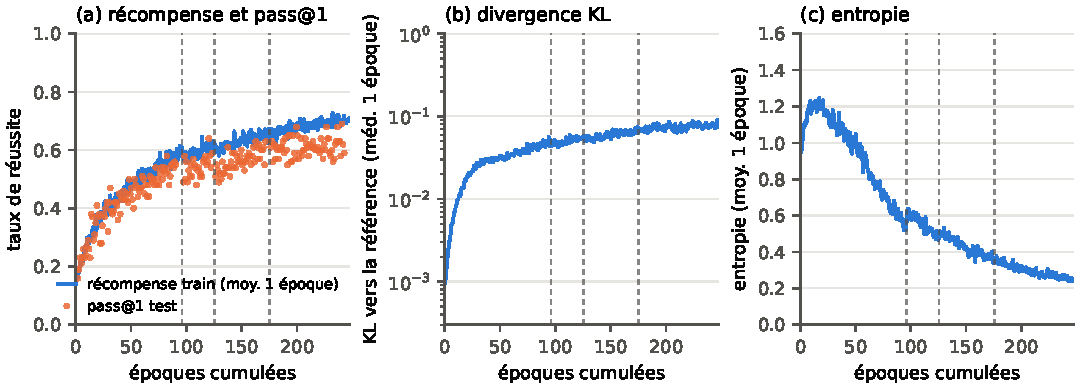
\includegraphics[width=\textwidth]{fig_fullft_stabilite.pdf}
\vspace{0.15cm}
\begin{keymsg}
Constat : la référence existe, mais elle est trop longue et trop coûteuse pour servir de base de travail. Il faut une porte vers l'efficience.
\end{keymsg}
\column{0.4\textwidth}
\begin{itemize}
  \item Hyperparamètres pris dans le code du papier.
  \item 40 \% à 30 époques, là où le papier annonce 75. \hl{69 \%} après 247 époques, plateau 61.
  \item Aucun collapse : KL lente et linéaire, entropie qui s'affûte.
  \item \hl{238 heures GPU}, 12 Go par sauvegarde. Impossible d'enchaîner des expériences.
\end{itemize}
\end{columns}
\end{frame}

% ---- 4a
\begin{frame}{Efficience : adaptation de rang faible (LoRA)}
\begin{columns}[T]
\column{0.5\textwidth}
\textbf{Pourquoi LoRA}
\begin{itemize}
  \item Adaptation de rang faible : une fraction des paramètres entraînés, l'optimiseur tient en mémoire.
  \item \emph{LoRA Without Regret} (2025) : en RL, LoRA égale le full finetuning. Hypothèse avancée : le RL n'apporte que quelques bits par épisode.
  \item Recette publiée : taux d'apprentissage dix fois plus élevé qu'en full finetuning.
\end{itemize}
\column{0.5\textwidth}
\textbf{Ce que ça change chez nous}
\begin{itemize}
  \item Adaptateur $r{=}8$ : 180 Mo au lieu de 12 Go par sauvegarde.
  \item Une mise à jour trois fois plus rapide, des grilles d'hyperparamètres possibles.
  \item Ancre KL naturelle : le modèle de base, adaptateur à zéro.
\end{itemize}
\end{columns}
\vspace{0.3cm}
\begin{center}\kpi{100}{$\times$ moins de mémoire d'optimiseur}\end{center}
\refs{Hu et al. 2022 (LoRA) ; Schulman et al. 2025 (LoRA Without Regret)}
\end{frame}

\begin{frame}{LoRA à référence fixe : dérive de la divergence KL}
\begin{columns}[T]
\column{0.58\textwidth}
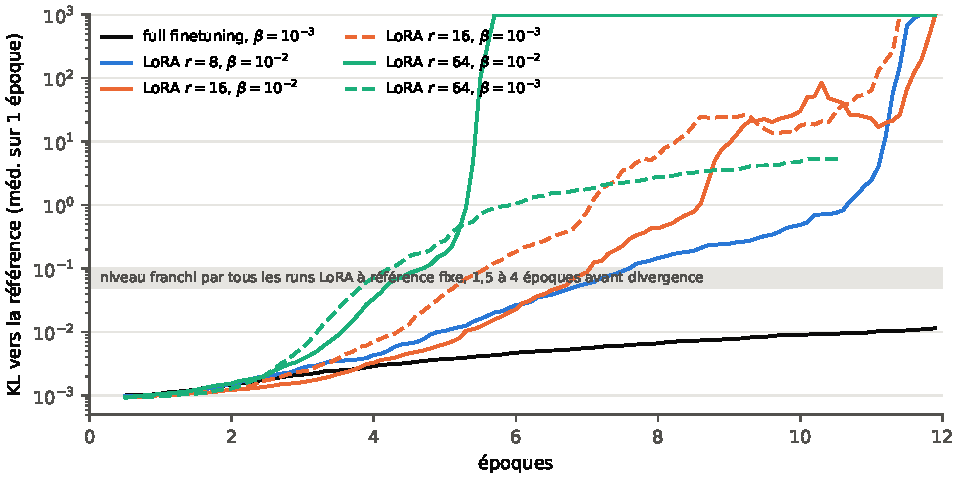
\includegraphics[width=\textwidth]{fig_kl_lora_vs_fullft.pdf}
\vspace{0.15cm}
\begin{keymsg}
Diagnostic : le frein KL n'engage qu'à KL $\approx 0{,}3$ pour $\beta=10^{-2}$. En régime sain, $\beta\cdot$KL vaut $10^{-5}$ contre $3\cdot10^{-3}$ pour le terme de politique. Il agit trop tard.
\end{keymsg}
\column{0.4\textwidth}
\small
\begin{itemize}
  \item Référence KL fixe = le modèle de base, comme dans le papier.
  \item Full finetuning : dérive \hl{linéaire}, $+10^{-3}$ par époque, stable sur 247 époques.
  \item LoRA, même référence : dérive \hl{géométrique}, $\times 5$ à $10$ toutes les deux époques, quel que soit le rang, le taux ou $\beta$. Tous franchissent 0,1 puis 1 en moins de quatre époques, puis collapse.
  \item $\beta$ retarde, le rang accélère, aucun réglage ne stabilise.
\end{itemize}
\end{columns}
\end{frame}

\begin{frame}{Correctif : référence KL mobile}
\begin{columns}[T]
\column{0.58\textwidth}
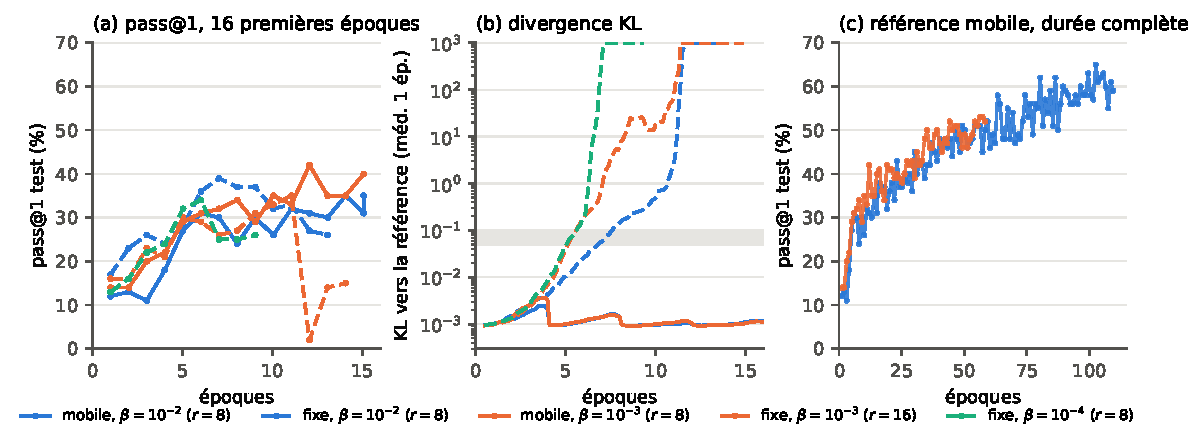
\includegraphics[width=\textwidth]{fig_anchor_square.pdf}
\column{0.4\textwidth}
\begin{itemize}
  \item Toutes les quatre époques : fusion de l'adaptateur, adaptateur vierge, référence = politique courante, optimiseur remis à zéro.
  \item La KL reste à $10^{-3}$ ; 65 puis \hl{73 \%}, au coût de LoRA.
  \item Croisement fixe/mobile $\times$ $\beta$ : c'est le régime de référence qui gouverne, pas $\beta$.
  \item Même idée retrouvée dans ProRL (réinitialisation de la référence et de l'optimiseur).
\end{itemize}
\end{columns}
\refs{Liu et al. 2025 (ProRL) ; Schulman et al. 2015 (TRPO, région de confiance)}
\end{frame}

\begin{frame}{Bilan de la stabilisation : deux modes de collapse}
\begin{columns}[T]
\column{0.58\textwidth}
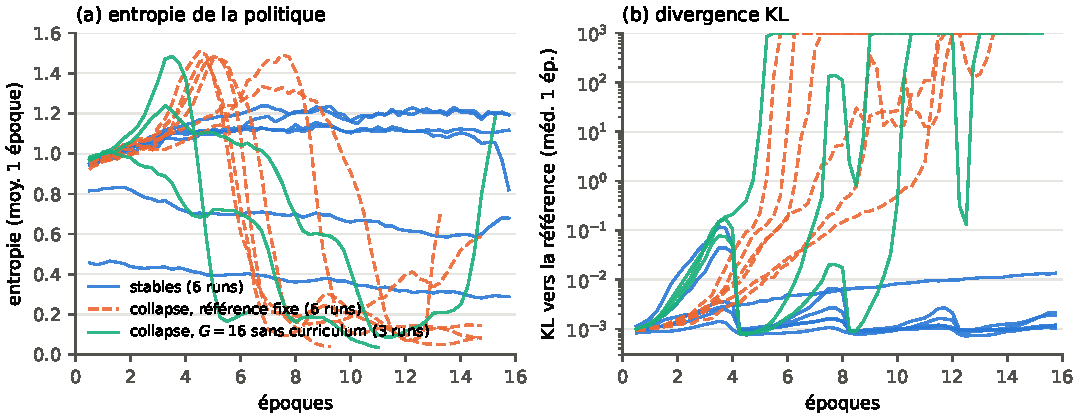
\includegraphics[width=\textwidth]{fig_collapse_signals.pdf}
\vspace{0.15cm}
\begin{keymsg}
Le second mode apparaît dès qu'on augmente la taille de groupe sans curriculum. C'est l'objet de la section suivante.
\end{keymsg}
\column{0.4\textwidth}
\footnotesize
Quinze runs, seize premières époques, classés par issue :
\begin{itemize}
  \item \textbf{6 stables} (bleu) : full-FT, ancre mobile $G{=}8$ à deux $\beta$, les trois curriculums.
  \item \textbf{6 collapses à référence fixe} (orange) : la grille LoRA. KL géométrique, entropie qui monte puis chute. \hl{La KL d'abord.}
  \item \textbf{3 collapses à $G{=}16$ sans curriculum} (vert) : contrôle, contrôle à ancre /12 époques, MAGELLAN. KL à $10^{-3}$, entropie qui décroît, puis tout casse. \hl{L'entropie d'abord.}
\end{itemize}
\end{columns}
\end{frame}

% ---- 4b

\begin{frame}{Trois régimes de curriculum à recette commune}
Recette commune : LoRA $r{=}8$, taux $3\cdot10^{-6}$, $\beta=10^{-2}$, ancre mobile toutes les quatre époques, $G=16$, 80 époques.
\vspace{0.2cm}
\begin{columns}[T]
\column{0.32\textwidth}
\begin{block}{Horizon}
Nombre de tours d'interaction : 10, puis 20, puis 30. Reprise de ScalingInter.
\end{block}
\column{0.32\textwidth}
\begin{block}{Budget}
Tokens par tour : 256, puis 512, puis 1024. Même famille, autre paramètre du harnais.
\end{block}
\column{0.32\textwidth}
\begin{block}{Profondeur}
Recettes de profondeur $\le 1$, puis $\le 2$, $\le 3$, $\le 4$. Palier suivant quand la récompense d'entraînement dépasse 0,8.
\end{block}
\end{columns}
\vspace{0.3cm}
\begin{itemize}
  \item Deux leviers : \hl{doser les moyens} (Horizon, Budget) ou \hl{ordonner les tâches} (Profondeur).
  \item Deux références sans curriculum : \textsc{Ancre-Mobile} à $G=8$ (73 \%) et \textsc{Contrôle-G16}, même recette que les curriculums.
\end{itemize}
\end{frame}

\begin{frame}{Calendriers des trois curriculums}
\begin{center}
\begin{tikzpicture}[x=0.135cm,y=0.85cm,font=\scriptsize]
  % axe des époques
  \draw[crMid,->] (0,-0.35) -- (82,-0.35) node[right,crDark] {époques};
  \foreach \e in {0,10,20,30,40,50,60,70,80} {\draw[crMid] (\e,-0.28) -- (\e,-0.42) node[below,crMid] {\e};}
  % Horizon
  \node[anchor=east,crDark,font=\small\bfseries] at (-1.5,2.3) {Horizon};
  \fill[crOrange!25] (0,2) rectangle (15,2.6);  \node at (7.5,2.3) {10 tours};
  \fill[crOrange!55] (15,2) rectangle (30,2.6); \node at (22.5,2.3) {20 tours};
  \fill[crOrange!90] (30,2) rectangle (80,2.6); \node[white] at (55,2.3) {30 tours};
  % Budget
  \node[anchor=east,crDark,font=\small\bfseries] at (-1.5,1.3) {Budget};
  \fill[crBlue!25] (0,1) rectangle (15,1.6);  \node at (7.5,1.3) {256 tokens};
  \fill[crBlue!55] (15,1) rectangle (35,1.6); \node at (25,1.3) {512 tokens};
  \fill[crBlue!90] (35,1) rectangle (80,1.6); \node[white] at (57.5,1.3) {1\,024 tokens par tour};
  % Profondeur (paliers adaptatifs, époques observées)
  \node[anchor=east,crDark,font=\small\bfseries] at (-1.5,0.3) {Profondeur};
  \fill[crDark!20] (0,0) rectangle (2.14,0.6);
  \fill[crDark!40] (2.14,0) rectangle (12.14,0.6); \node at (7.2,0.3) {$d\le2$};
  \fill[crDark!60] (12.14,0) rectangle (22.14,0.6); \node[white] at (17.2,0.3) {$d\le3$};
  \fill[crDark!85] (22.14,0) rectangle (80,0.6); \node[white] at (51,0.3) {$d\le4$ : toutes les recettes};
  \node[anchor=south,crDark] at (1.1,0.62) {$d\le1$};
\end{tikzpicture}
\end{center}
\footnotesize
\begin{itemize}\setlength{\itemsep}{1pt}
  \item \textsc{Horizon}, \textsc{Budget} : paliers fixés, longs, pour laisser chaque niveau saturer (le papier change toutes les 100 mises à jour, deux époques environ).
  \item \textsc{Profondeur} : palier suivant dès que la récompense d'entraînement dépasse 0,8 sur une époque, ou après 10 époques. Observé : 2,1, 12,1, 22,1. La version à calendrier fixe (0, 12, 25, 37) saturait : six époques sans gradient au palier 1.
  \item Un palier change : l'épisode tronqué (Horizon), la réponse tronquée (Budget), les tâches échantillonnées (Profondeur).
\end{itemize}
\end{frame}

\begin{frame}{Mécanisme proposé : groupes mixtes et entropie}
\begin{itemize}
  \item Seuls les groupes \emph{mixtes} produisent du gradient. Sans curriculum, à trente tours, les tâches difficiles sont mixtes dès le début.
  \item Dans un tel groupe : une réussite courte et routinière (\hl{exploitation}, renforcée) contre quinze échecs longs pleins d'actions rares (\hl{exploration}, punie token par token).
  \item Cui et al. 2025 : l'entropie baisse quand le probable est récompensé et l'improbable puni. Rien ne la recharge. Au plancher, la politique se fige, puis la KL part.
  \item Un curriculum décide \emph{quand} une tâche a le droit de produire du gradient : les tâches hors de portée ne punissent pas, les échecs sont courts, les réussites du palier suivant viennent d'actions rares.
\end{itemize}
\vspace{0.3cm}
\begin{keymsg}
Hypothèse cohérente avec toutes nos courbes. Deux maillons ne sont pas mesurés directement : la composition des groupes mixtes et le signe de la covariance de Cui et al. sur nos runs.
\end{keymsg}
\refs{Cui et al. 2025 (The Entropy Mechanism of RL for Reasoning LMs)}
\end{frame}

\begin{frame}{Résultats des curriculums : pass@1 et entropie}
\begin{columns}[T]
\column{0.58\textwidth}
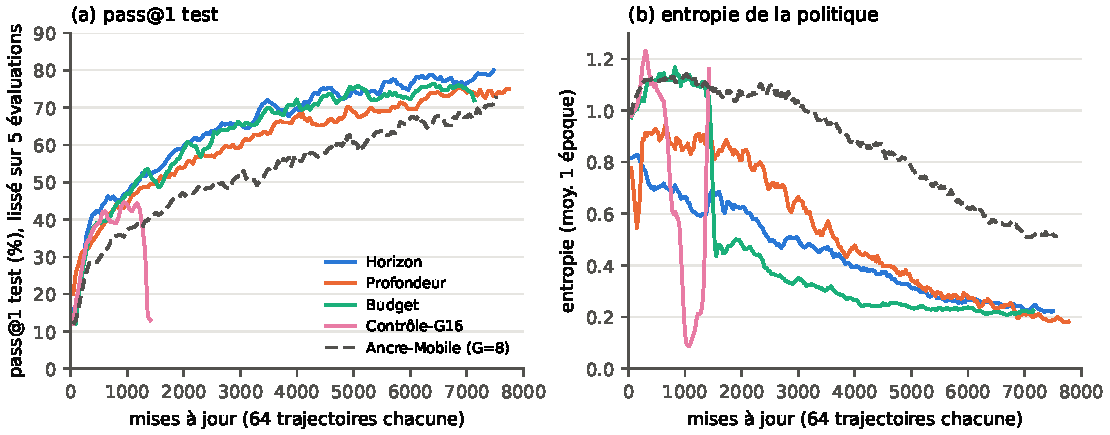
\includegraphics[width=\textwidth]{fig_curricula_pass1_entropy.pdf}
\column{0.4\textwidth}
\footnotesize\setlength{\tabcolsep}{4pt}
\begin{tabular}{@{}lrr@{}}
\toprule
 & plateau & meilleur \\
\midrule
\textsc{Horizon} & \textbf{78} & \textbf{82} \\
\textsc{Budget} & 75 & 80 \\
\textsc{Profondeur} & 74 & 80 \\
\textsc{Ancre-Mobile} $G{=}8$ & 70 & 73 \\
\textsc{Réplication-FT} & 61 & 69 \\
\textsc{Contrôle-G16} & \multicolumn{2}{c}{54 puis collapse} \\
\bottomrule
\end{tabular}
\vspace{0.2cm}
\begin{itemize}\setlength{\itemsep}{2pt}
  \item Le contrôle meurt à l'époque 10 ; les trois curriculums tiennent 80 époques.
  \item L'entropie des curriculums descend plus bas que celle de la référence $G{=}8$, mais sur 60 époques et avec un pass@1 qui monte : un affûtage, pas un effondrement.
  \item Papier : 75. Incertitude d'une évaluation : environ 3 points.
\end{itemize}
\end{columns}
\end{frame}

\begin{frame}{Résultats par profondeur et par classe d'erreur}
\begin{columns}[T]
\column{0.5\textwidth}
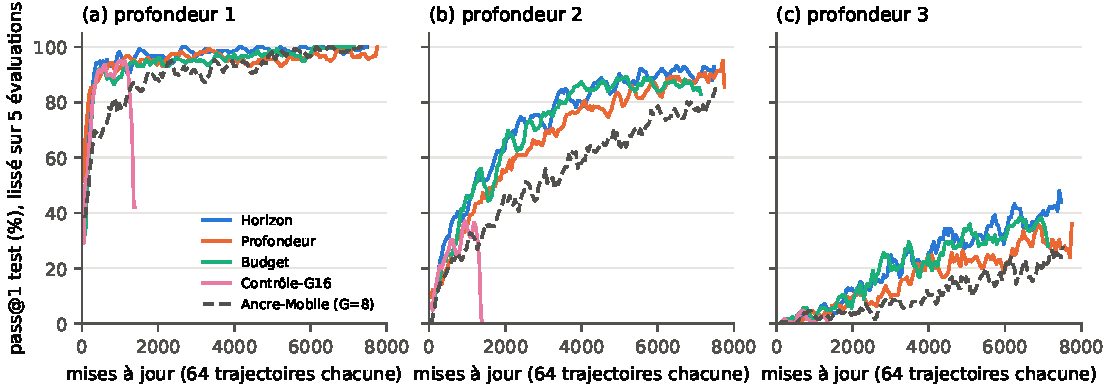
\includegraphics[width=\textwidth]{fig_curricula_depths.pdf}
\column{0.5\textwidth}
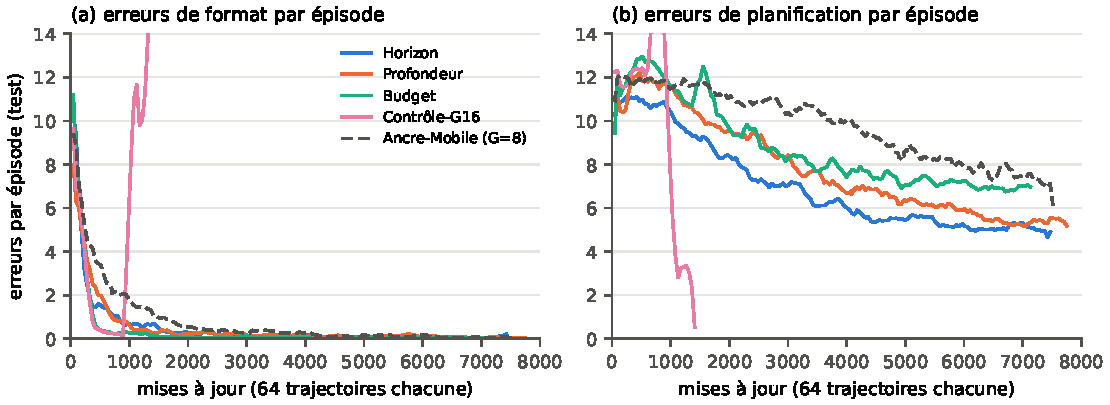
\includegraphics[width=\textwidth]{fig_curricula_errors.pdf}
\end{columns}
\vspace{0.2cm}
\begin{itemize}
  \item Profondeur 1 acquise en cinq époques, profondeur 2 vers 90 \%, profondeur 3 entre 30 et 45 \%, profondeur 4 jamais.
  \item Les curriculums accélèrent sans changer l'ordre d'acquisition. Erreurs de forme éliminées en moins de mille mises à jour ; erreurs de planification lentes.
\end{itemize}
\end{frame}


% =====================================================================
\section{Conclusion et perspectives}

\begin{frame}{Contributions}
\begin{enumerate}
  \item \textbf{Un cadrage.} D'un sujet ouvert sur l'auto-amélioration à une question précise : les conditions de stabilité et d'efficience du RL multi-tour, une fois l'environnement donné. Une synthèse de la littérature organisée autour de cette question.
  \item \textbf{Une réplication à conditions égales} de la recette publiée sur un seul GPU, et une recette LoRA qui tient : l'ancre KL mobile. 69 \% en full finetuning, \hl{73 \%} en LoRA au dixième du coût.
  \item \textbf{Deux modes de collapse} caractérisés sur quinze runs, la KL d'abord ou l'entropie d'abord, avec un mécanisme proposé au niveau du gradient.
  \item \textbf{Le curriculum comme protection}, à recette identique et compute contrôlé : trois régimes qui tiennent là où le contrôle casse, jusqu'à \hl{82 \%} pour 75 dans le papier.
\end{enumerate}
\vspace{0.2cm}
\begin{keymsg}
Et une infrastructure reproductible : entraînement, évaluation, journaux et recettes, prête à être réutilisée sur un autre environnement.
\end{keymsg}
\end{frame}

\begin{frame}{Périmètre de validité et perspectives}
\footnotesize
\begin{columns}[T]
\column{0.48\textwidth}
\textbf{Ce que les résultats autorisent}
\begin{itemize}
  \item Des comparaisons \emph{internes}, à recette identique et compute mesuré.
  \item Des conditions de stabilité indépendantes du modèle : masquage, récompense, régime de référence, dosage de la difficulté.
\end{itemize}
\textbf{Ce qu'ils n'autorisent pas}
\begin{itemize}
  \item Un run par configuration ; un environnement, un modèle de 3B, un GPU.
  \item L'écart à budget égal avec le papier reste inexpliqué.
  \item $G$, tâches par pas et fréquence d'ancre ne sont pas séparés (annexe B4).
\end{itemize}
\column{0.5\textwidth}
\textbf{Ce que les résultats appellent}
\begin{itemize}
  \item Rééquilibrer le jeu d'entraînement par profondeur ; une seule recette de profondeur 4.
  \item Répéter les runs décisifs avec plusieurs graines.
  \item Éprouver ancre mobile et curriculums sur les autres environnements d'AgentGym-RL, puis sur l'environnement d'achat de Criteo, où la récompense n'est ni binaire ni exacte.
\end{itemize}
\textbf{Ce qu'ils ouvrent}
\begin{itemize}
  \item Combiner les leviers de curriculum ; leurs effets ne s'additionnent pas forcément.
  \item Faire choisir la difficulté par le modèle, sur une base stabilisée, là où elle n'est pas connue à l'avance.
\end{itemize}
\end{columns}
\end{frame}


{
\setbeamercolor{background canvas}{bg=crDark}
\setbeamertemplate{footline}{}
\begin{frame}[plain]
  \vfill
  \begin{center}
    {\color{crOrange}\rule{2.4cm}{3pt}}\\[0.6cm]
    {\color{white}\fontsize{26}{30}\selectfont\bfseries Merci.\par}
    \vspace{0.4cm}
    {\color{white}\large Questions ?\par}
    \vspace{1cm}
    {\color{crMid}\small Rapport, code, recettes et journaux : dépôt \texttt{rl-gym-workout}}
  \end{center}
  \vfill
\end{frame}
}

% =====================================================================
\appendix
\inappendixtrue
\section{Annexe}

\begin{frame}{B1. SNIS : recombinaison de trajectoires intra-groupe}
\begin{itemize}
  \item Idée : dans un groupe, une pensée $z_j$ et une réponse $a_i$ venues de trajectoires différentes forment un couple valide. Repondérer chaque couple par un poids d'importance auto-normalisé.
  \[ \tilde w_{ij} = \frac{\pi_\theta(a_i \mid x, z_j)}{\sum_{l} \pi_\theta(a_i \mid x, z_l)} \]
  \item Estimateur biaisé à $G$ fini, consistant, variance réduite (Owen, chap. 9).
  \item En multi-tour, la recombinaison casse la cohérence causale entre observation et action : effondrement observé (exp17), arrêté.
\end{itemize}
\refs{Annexe B du rapport ; Owen 2013 ; Kazemnejad et al. 2024 (VinePPO)}
\end{frame}

\begin{frame}{B2. Planification mono-tour et contrôle multi-tour}
\begin{itemize}
  \item Qwen3.5-4B : 54 \% en plan complet rejoué, 77 \% en interactif. \hl{La boucle de rétroaction vaut 23 points.}
  \item Politique RL interactive : planification 12 $\to$ 19,5 \% sur onze températures. Transfert réel mais faible : ce que le RL a appris est surtout réactif.
  \item RL de planification pure : 37 \% en plan, 9 \% en interactif. Détruit le protocole une action par tour.
  \item Non testé : l'alternance des deux régimes.
\end{itemize}
\refs{Annexe D ; Dupoux, LeCun et Malik 2026}
\end{frame}

\begin{frame}{B3. MAGELLAN : autocurriculum par progrès d'apprentissage}
\begin{itemize}
  \item Tête de compétence sur l'état caché du modèle, adaptateurs dédiés ; progrès = $|$prédiction $-$ prédiction retardée$|$ ; échantillonnage proportionnel au progrès.
  \item Prédiction écrite avant le run : désinvestir la profondeur 4. Vérifiée : $p(d_4)=0{,}0006$ en fin de run.
  \item 45 \% à l'époque 6, collapse aux époques 7 et 8, plus tôt que le contrôle.
  \item Le progrès mesure du changement ; un collapse est un changement. L'estimateur a concentré 79 \% de l'échantillonnage sur la profondeur 1 et accéléré la panne.
  \item Condition d'emploi : un apprenant stable. Suite naturelle : le brancher sur une recette stabilisée par curriculum.
\end{itemize}
\refs{Gaven et al. 2025 ; Graves et al. 2017 ; annexe E}
\end{frame}

\begin{frame}{B4. Contrôle complémentaire : $G{=}16$, huit tâches par pas}
\begin{columns}[T]
\column{0.6\textwidth}
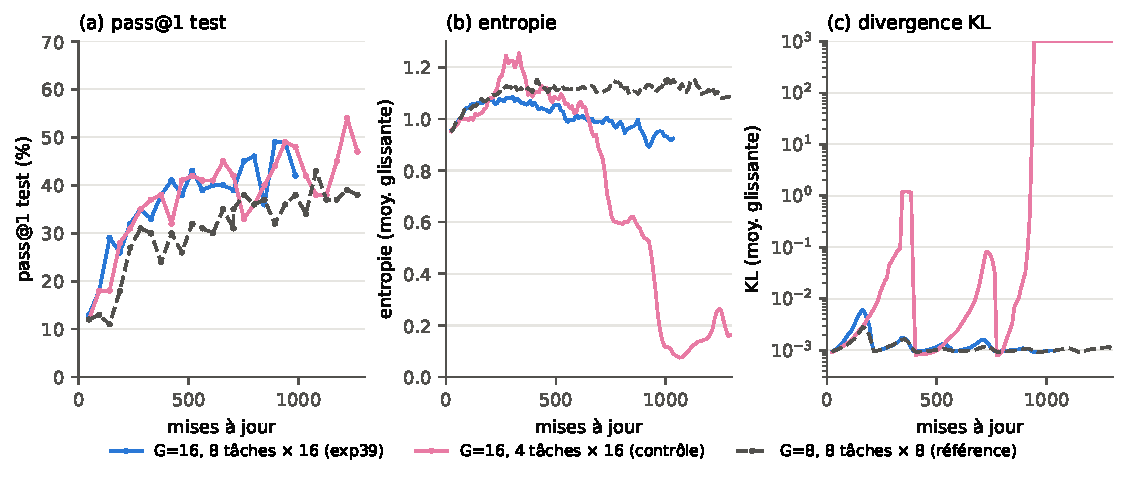
\includegraphics[width=\textwidth]{fig_exp39_control.pdf}
\column{0.38\textwidth}
\small
\begin{itemize}
  \item Stable à l'époque 22 : KL $10^{-3}$, entropie 1,05 $\to$ 0,93, pass@1 49.
  \item Face à la référence $G{=}8$ : un seul écart, $G$. Donc $G{=}16$ seul ne suffit pas à effondrer un run.
  \item Face au contrôle : deux écarts. Huit tâches au lieu de quatre, \emph{et} ré-ancrage tous les 184 pas au lieu de 372, l'ancre étant définie en époques.
  \item Le run propre : même chose avec ancre toutes les huit époques.
\end{itemize}
\end{columns}
\end{frame}

\begin{frame}{B5. L'estimateur pass@$k$ et l'oracle par profondeur}
\begin{itemize}
  \item Chen et al. 2021 : avec $n$ tirages et $c$ succès, $\widehat{\text{pass@}k} = 1 - \binom{n-c}{k}\big/\binom{n}{k}$. Sans biais, contrairement au « meilleur de $k$ » sur un seul lot.
  \item 3B nu : pass@1 10,3 ; pass@20 47. Profondeur 2 : 44 \% atteignable. Profondeurs 3 et 4 : 0 sur 500 et 0 sur 60 tirages.
  \item Un modèle entraîné modestement (32 \%) résout à 20 tirages 14 tâches de profondeur 2 et 2 de profondeur 3 que le modèle nu ne résolvait jamais : pass@20 65.
  \item \textsc{Horizon} : pass@1 82, au-dessus du pass@20 du modèle nu. Mise en tension de la thèse du plafond, pas réfutation : $k=20$ est petit, et le RL de Yue et al. est court.
\end{itemize}
\end{frame}

\begin{frame}{B6. Incertitude d'une évaluation}
\begin{itemize}
  \item 100 tâches, tirage de Bernoulli chacune : $\sigma = \sqrt{p(1-p)/100} \le 5$ points. Borne haute.
  \item Stratifié par profondeur : $\sigma^2 = \sum_d n_d\, p_d(1-p_d)/100^2$, soit 3,1 à 3,4 points sur nos runs. Observé entre évaluations successives : 2,2 à 2,6.
  \item Le meilleur score d'une courbe est un maximum sur environ 150 évaluations : biaisé vers le haut. D'où le plateau comme chiffre de tête.
  \item Zéro-shot : 18 en une passe, 10,3 en moyenne de vingt. Le 18 était un tirage chanceux.
\end{itemize}
\end{frame}

\begin{frame}{B7. Divergence KL par run et effet de $\beta$}
\scriptsize
\begin{tabular}{@{}lccccl@{}}
\toprule
Run & référence & $\beta$ & KL ép. 4-6 & KL ép. 8-10 & issue \\
\midrule
Full-FT & fixe & $10^{-3}$ & 0,004 & 0,008 & stable, 0,08 à 247 ép. \\
LoRA r16 & fixe & $10^{-3}$ & 0,040 & 17,7 & collapse ép. 8-10 \\
LoRA r16 & fixe & $10^{-2}$ & 0,007 & 8,0 & collapse ép. 8-10 \\
LoRA r8 & fixe & $10^{-2}$ & 0,010 & 0,26 & collapse ép. 11 \\
LoRA r8 & fixe & $10^{-4}$ & 0,047 & $10^{12}$ & divergence ép. 6-8 \\
LoRA r8 & mobile & $10^{-2}$ & 0,001 & 0,001 & stable 111 ép., 73 \\
LoRA r8 & mobile & $10^{-3}$ & 0,001 & 0,001 & stable 60 ép., 53 \\
\bottomrule
\end{tabular}
\vspace{0.3cm}
\small
\begin{itemize}
  \item $\beta=10^{-2}$ et $10^{-3}$ indiscernables à référence mobile : 48,9 contre 49,7 aux époques 49-58.
  \item La bande 0,05-0,1 n'est pas universelle : le full finetuning y vit stablement ; des runs à ancre mobile la dépassent transitoirement puis reviennent.
\end{itemize}
\end{frame}

\begin{frame}{B7b. Pics de KL : l'estimateur $k_3$ n'est pas borné dans TRL}
\begin{columns}[T]
\column{0.6\textwidth}
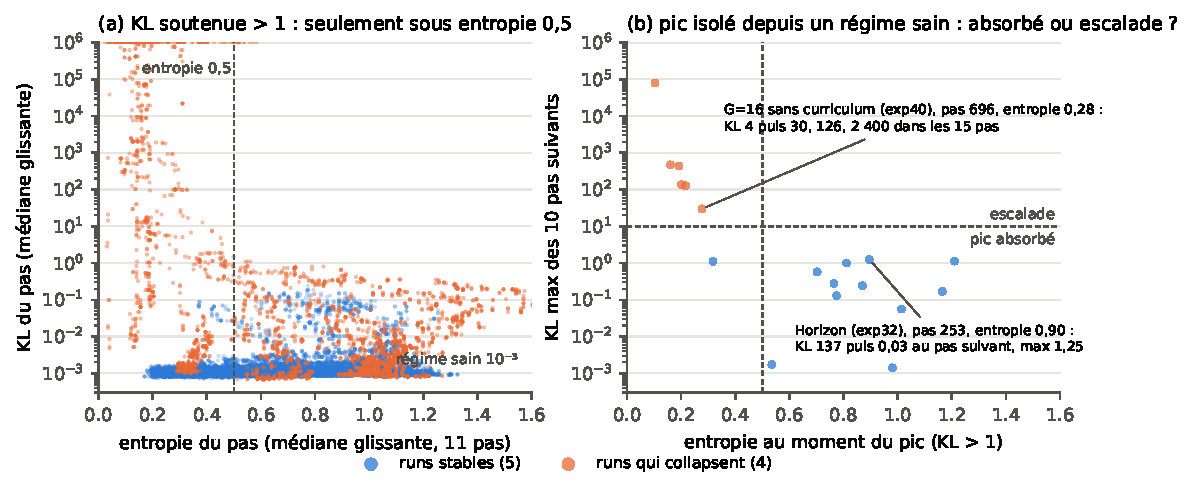
\includegraphics[width=\textwidth]{fig_collapse_entropy_kl.pdf}
\column{0.38\textwidth}
\small
\begin{itemize}
  \item KL loguée $= \overline{k_3}$ sur les tokens tirés, $k_3 = e^{\rho}-\rho-1$, $\rho = \log\pi_{\mathrm{ref}} - \log\pi$. verl borne $k_3$ à 10 par token ; \hl{TRL ne borne pas}.
  \item (a) Neuf runs : une KL soutenue $> 1$ n'apparaît que sous une entropie de 0,5 ; nécessaire, pas suffisant (\textsc{Horizon} vit 20 époques à 0,25).
  \item (b) Dix-huit pics isolés : 12 à entropie $> 0{,}5$, tous absorbés ; 6 à entropie $< 0{,}3$, tous en escalade.
  \item Rejeu token par token du contrôle $G{=}16$, 5 pas avant l'explosion (pas 705, 256 épisodes) : tours médians de 12 tokens, 81 \% commencent par « Action ». Les plus gros $k_3$ (300) sont des « Thought » tirés à $p = 0{,}3\,\%$ là où la référence en donne 0,6 : $\rho \approx 5$. Après l'explosion (pas 846) : 100 \% du $k_3$ sur les \texttt{<|im\_end|>} forcés des tours en boucle tronqués, $\rho = 45$, $k_3 = 10^{19}$.
  \item Lecture : l'entropie s'effondre d'abord ; l'explosion de KL est un artefact de $k_3$ non borné sur des tokens que la politique a éliminés. Ni tirage de queue vLLM, ni écart vLLM/HF (médiane $10^{-5}$ nat).
\end{itemize}
\end{columns}
\end{frame}

\begin{frame}{B8. Divergences entre le texte et le code du papier}
\begin{itemize}
  \item Texte : 20 tours d'interaction. Code : 30, à l'entraînement comme à l'évaluation. Nous suivons le code.
  \item Script publié : 32 tâches $\times$ 8 trajectoires par collecte, 4 pas clippés de 64, 30 rounds. Le texte dit 20 rounds. Aucun nombre d'époques nulle part.
  \item Une seule configuration, celle du 7B. Le 3B est un score sans recette.
  \item Notre choix de 64 trajectoires et un pas par collecte : ratio d'importance $\equiv 1$, clipping inerte, une politique fraîche à chaque mesure. Un mécanisme à la fois. Passer à 256 en quatre pas ajoute une région de confiance : job écrit, pas lancé.
\end{itemize}
\end{frame}

\begin{frame}{B9. Compute par lignée}
\small
\begin{tabular}{@{}lrrrrr@{}}
\toprule
 & mises à jour & h GPU & tokens & tours env. (est.) & plateau \\
\midrule
\textsc{Réplication-FT} & 11\,564 & 238 & 0,87 G & 12,4 M & 61 \\
\textsc{Ancre-Mobile} $G{=}8$ & 8\,018 & 70 & 0,62 G & 8,6 M & 70 \\
\textsc{Horizon} & 7\,518 & 48 & 0,45 G & 6,3 M & 78 \\
\textsc{Budget} & 7\,194 & 51 & 0,43 G & 7,2 M & 75 \\
\textsc{Profondeur} & 7\,904 & 66 & 0,56 G & 7,9 M & 74 \\
\textsc{Contrôle-G16} & 1\,434 & 16 & 0,15 G & 1,9 M & collapse \\
\bottomrule
\end{tabular}
\vspace{0.3cm}
\begin{itemize}
  \item Tours d'environnement estimés à partir du nombre de tours moyen par profondeur et par palier.
  \item Les curriculums de moyens coupent les épisodes : moins chers par pas.
\end{itemize}
\end{frame}

\begin{frame}{B10. Effet de la génération du modèle de base}
\begin{itemize}
  \item Qwen3.5-4B sans entraînement : \hl{78,5 \%} en moyenne de 18 passes, 97 \% de pass@18. Un an après Qwen2.5.
  \item Notre 82 \% après entraînement est presque atteint sans RL par la génération suivante.
  \item Ce qui ne dépend pas du modèle : les conditions qui font réussir ou échouer l'entraînement. Masquage, récompense, régime de référence, dosage de la difficulté.
  \item Sur un environnement propriétaire, où aucun modèle n'a été pré-entraîné, ce sont ces conditions qui comptent.
  \item Mesure manquante : un run court de la recette stabilisée sur Qwen3.5-4B.
\end{itemize}
\end{frame}

\begin{frame}{B11. Écart avec les résultats publiés}
\begin{itemize}
  \item À recette identique et budget d'époques comparable : 40 \% chez nous, 75 annoncés.
  \item Ce qu'on sait : le 3B n'a pas de recette publiée ; texte et code divergent ; aucune incertitude n'est donnée ; leur collecte de 256 en quatre pas clippés ajoute une région de confiance que notre recette on-policy n'a pas.
  \item Ce qu'on ne sait pas : laquelle de ces différences porte l'écart. Le rapport le dit, il ne le résout pas.
  \item En deux phrases : nous n'avons pas reproduit leur chiffre à leur budget, et nous l'avons dépassé à un budget deux fois et demie supérieur, avec une recette dont chaque élément est documenté.
\end{itemize}
\end{frame}

\begin{frame}{B12. Prompt few-shot}
\begin{itemize}
  \item Des exemples de trajectoires réussies dans le prompt, tirés du réservoir de 70 recettes sans fuite.
  \item Gain immédiat sur le modèle nu, avant tout entraînement.
  \item Interaction few-shot et RL testée dans une configuration antérieure à la recette stabilisée, non refaite depuis.
\end{itemize}
\refs{Brown et al. 2020 ; section 4.5 du rapport}
\end{frame}

\begin{frame}{B13. Objectif GRPO}
\begin{itemize}
  \item Objectif clippé de PPO, avantage de groupe à la place d'une fonction de valeur :
  \[ \mathcal L = -\frac{1}{G}\sum_{i}\frac{1}{|o_i|}\sum_{t} \min\!\Big(r_{i,t}\hat A_i,\ \operatorname{clip}(r_{i,t},1-\epsilon,1+\epsilon)\hat A_i\Big) + \beta\, \mathrm{KL}(\pi_\theta \,\|\, \pi_{\text{ref}}) \]
  \item Strictement on-policy chez nous : $r_{i,t}\equiv 1$, le clipping est inerte.
  \item Masque d'environnement : les tokens d'observation ont un poids nul dans la somme sur $t$, mais restent dans le contexte.
  \item Dr.~GRPO : la normalisation par la longueur et par l'écart-type introduit des biais. Nous gardons la normalisation par l'écart-type ; les runs se comparent à recette identique.
\end{itemize}
\end{frame}

\begin{frame}{B14. Réorientation initiale : de la recommandation aux agents}
\begin{itemize}
  \item Intégration aux équipes Criteo : état de l'art en recommandation, publicités conversationnelles, identifiants sémantiques.
  \item Constat : la littérature de recommandation est mono-tour, statique, sans outils. Le pont direct vers des agents interactifs multi-tour était prématuré pour six mois.
  \item Réorientation délibérée vers l'étude fondamentale de l'auto-apprentissage des agents, sur un cadre académique reproductible.
  \item Ce que Criteo en retire : une synthèse structurée, une brique technique réutilisable, et les conditions d'un entraînement qui réussit.
\end{itemize}
\refs{Annexe C.1 du rapport}
\end{frame}

\end{document}
